% Requires running Bibtex

\documentclass[%
reprint,
amsmath,amssymb,
aps,
]{revtex4-2}

\usepackage{graphicx}% Include figure files
\usepackage{dcolumn}% Align table columns on decimal point
\usepackage{bm}% bold math
\usepackage{hyperref}% add hypertext capabilities
\usepackage[font=small,labelfont=bf,justification=justified,format=plain]{caption}% change fontsize in captions
\usepackage{booktabs}% cool table style
\hypersetup{
	colorlinks=true,       % false: boxed links; true: colored links
	linkcolor=black,        % color of internal links
	citecolor=black,        % color of links to bibliography
	filecolor=black,     % color of file links
	urlcolor=black         
}

\begin{document}
	
	\preprint{APS/123-QED}
	
	\title{PHYC30170 Physics with Astronomy and Space Science Lab 1;\\Astronomical Image Analysis}% Force line breaks with \\
	
	\author{Daragh Hollman}
	\email{daragh.hollman@ucdconnect.ie}
	
	\date{\today}
	
	\begin{abstract}
		An article usually includes an abstract, a concise summary of the work
		covered at length in the main body of the article. 
	\end{abstract}

	\maketitle
	
	\section{Introduction}

		Astronomical image analysis is fundamental to the understanding...
	
	
	\section{Theory}
	
		This is the theory section.
	
		\subsection{Image Reduction}
			When taking images in astronomy there exists a level of background noise and non-uniformities which must be accounted for to ensure accurate measurements. Removing these effects is known as data reduction\cite{manual}. This noise comes from many things including readout electronics, thermal emissions, and non-uniformities in the detector\cite{astropy}. To ameliorate some of these noises and remove non-uniformities, flat field and bias frames are taken. Flat field frames (flats) are controlled, uniformly illuminated images used to correct for non-uniformities in the detector. Bias frames (biases) are images taken with a near (ideally exactly) zero second exposure time. These are used to ameliorate noise due to readout electronics. They contain no light and hence provide a constant offset which can be subtracted from all further images. Signals due to thermal emissions can be accounted for by keeping the imaging device cool.\\
		
		\subsection{Apparent Size}
			To find the size of the galaxy...\\
			
			
			The apparent size of the source can be determined using trigonometry using \ref{eq:arctan} as shown in figure \ref{fig:trig}.
			\begin{equation}
				\theta = 2 \arctan{\left(\frac{d}{2 D}\right)}
				\label{eq:arctan}
			\end{equation}where $\theta$ is the angular size, $d$ is the apparent size and $D$ is the distance between the source and the observer. This equation can be rearranged to get an expression for the angular size using the small angle approximation.
			\begin{equation}
				d = \frac{\theta}{206265\,\text{arcsec}} D
				\label{eq:angSize}
			\end{equation}The scalar divisor is introduced to work with $\theta$ in units of arcseconds as there are approximately 206265 arcseconds in a radian\cite{modernAstro}.
		
		\subsection{Aperture Photometry}
		
			\begin{equation}
				m_{std} = -2.5 \, \log_{10}\left(\frac{F}{t}\right) + \text{ZP}
				\label{eq:mag}
			\end{equation} where $m_{std}$ is the calibrated magnitude of a source in the system, $F$ is the measured background-subtracted counts from the light source, $t$ is the exposure time and $\text{ZP}$ is the zeropoint for the image.\\
		
			Do some talking about what the zeropoint actually is.\\
			
			Rearranging equation \ref{eq:mag} for $\text{ZP}$:
			
			\begin{equation}
				\text{ZP} = m_{std} + 2.5 \log_{10}\left(\frac{F}{t}\right)
				\label{eq:zeropoint}
			\end{equation}
		
		\subsection{CCD}
		
			A CCD is used...\\
			
			Signal to noise (which can be compared to the fits file data)...\\
			
			\begin{equation}
				\frac{S}{N} = \frac{F_\star}{\sqrt{F_\star + n_\star \left( 1 + \frac{n_\star}{n_\text{sky}}\right) \times \left(F_\text{sky} + R^2\right)}}
			\end{equation}where $\frac{S}{N}$ is the signal noise ratio, $F_\star$ and $F_\text{sky}$ are the number of counts measured from the source and the background annulus respectively, $n_\star$ and $n_\text{sky}$ are the number of pixels within the  
	 
	\section{Methodology}
	
		The images analysed in this experiment were taken by the IAC 80 Telescope at the Teide Observatory on Tenerife. The two objects analysed were Messier 91 (M91), a barred spiral galaxy\cite{messier}, and NN Serpentis (NN Ser), a post-main sequence eclipsing binary\cite{Horner_2012}. 63 images of M91 were taken, 21 biases, 11 flat field images were taken in 3 filters B, V and H$\alpha$ and 9 images of the object itself were taken divided between the 3 filters. 46 images were taken of NN Ser. 21 biases, 7 flats and 18 object images, all in the clear band. The images were all in FITS file formatting and were handled in python using the \texttt{ASTROPY} package.
	
		\subsection{Data Reduction}
			
			 For both the M91 and NN Ser images, the bias files and the flat files were averaged element-wise to create a master bias file which was an average of all the bias files. This was similarly done for the flat files in each band, however the master bias was subtracted from each flat image beforehand. Using these master files, each object image was then reduced by subtracting the master bias and diving by the master flat.
		
		\subsection{Determining the Size of Messier 91}
			
			\subsubsection{Angular Size}
			
				As the images for M91 were taken in three different bands, these reduced images were first combined to create an averaged image in each band and were then added together to create a deeper image. To determine the angular size, the size of the galaxy in pixels needed to be calculated. This was done by iterating through the image in buckets of 5$\times$5 pixels. The average counts in this bucket was compared to an average background count over a region of 250$\times$250 pixels which was definitely outside of the galaxy. If the bucket counts were greater than the background counts by a certain tolerance, (a tolerance of 22 counts was chosen in this case as it visually fit the galaxy well), it was recorded as a bright bucket. This tolerance factor was used to estimate uncertainty on the angular size by using a higher and lower value to calculate larger and smaller angular sizes.\\
				
				The algorithm searched for the largest number of sequential bright buckets as that would represent the angular size of the galaxy in pixels. This was calculated for both the X and Y axes of the image to account for a major and minor size. It is important to note that the image was not aligned such that the X and Y axes were parallel to the major and minor axes of the galaxy, and although in this report we will refer to a major and a minor axis, these are not indicative of the galaxy's physical major and minor axes. The angular distance per pixel and the distance to the galaxy were known and hence the angular size was calculated using equation \ref{eq:angSize}.
			
			\subsubsection{Adjusting for Inclination and Position Angle}
				Talk about how you did this when you do it I guess.
		
		\subsection{Measuring Photometry of NN Serpentis and Plotting its Lightcurve}
			
			\subsubsection{Calibrating to the r Filter and Determining Zeropoint}
				To measure the magnitude of NN Serpentis, aperture photometry is used. To calculate the zeropoint equation \ref{eq:zeropoint} was used. A set of stars and reference magnitudes was required to calibrate this. The magnitude data most available was measured in the r filer and hence the system was calibrated from the clear filter to the r filter. Four stars nearby NN Ser with known magnitudes in the r filter were selected to calibrate the system\cite{parsons}. These stars are identified in figure \ref{fig:rBandStars}
				
				\begin{figure}
					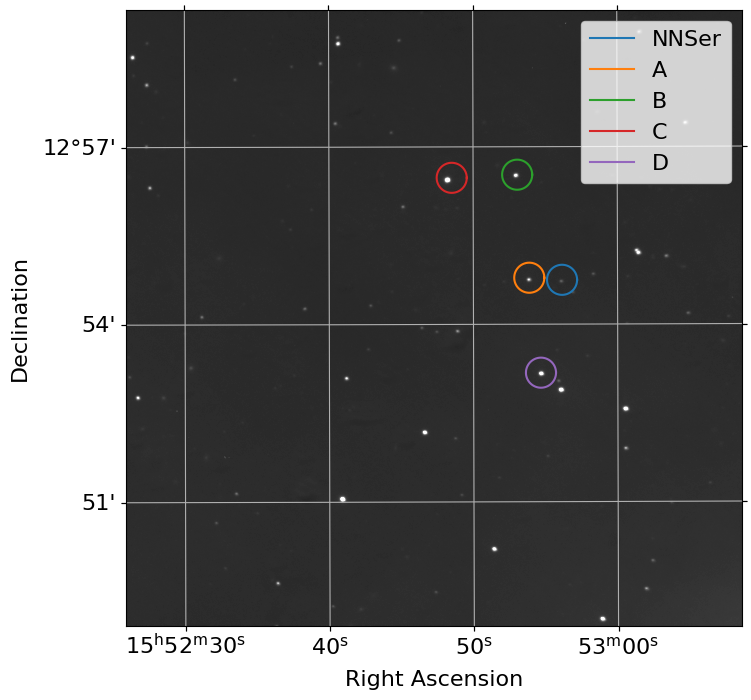
\includegraphics[width=\columnwidth]{rBandStars.png}
					\caption{\label{fig:rBandStars} An image of NN Serpentis. The reference stars used to calibrate the system to the r filter are circled to identify them.}
				\end{figure}
			
				\begin{table}[]
					\begin{tabular*}{0.8\linewidth}{@{\extracolsep{\fill}}llll@{}}
						\toprule
						Star & r'   & \begin{tabular}[c]{@{}l@{}}RA offset\\ (arcsec)\end{tabular} & \begin{tabular}[c]{@{}l@{}}Dec. offset\\ (arcsec)\end{tabular} \\ \midrule
						A    & 15.8 & -31.4                                                        & +2.2                                                           \\
						B    & 15.1 & -46.4                                                        & +106.7                                                         \\
						C    & 13.7 & -114.5                                                       & +103.7                                                         \\
						D    & 13.7 & -22.2                                                        & -94.1                                                          \\ \bottomrule
					\end{tabular*}
					\caption{A table of the reference stars used reference stars used to calibrate the system to the r filter\cite{parsons}. The coordinate offset is with respect to NN Serpentis.}
					\label{tab:pearsons}
				\end{table}
			
			\subsubsection{Aperture Photometry of NN Serpentis}
		
	\section{Results}
	
		\subsection{Messier 91}
		
			The angular size is plotted as an ellipse in figure \ref{fig:angSize}
			
			\begin{figure}
				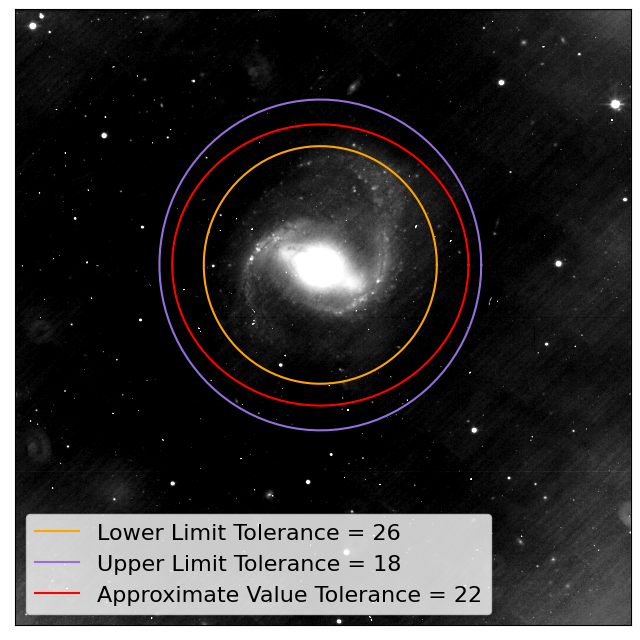
\includegraphics[width=\columnwidth]{angularSize.png}
				\caption{\label{fig:angSize} The reduced and combined image of Messier 91 with ellipses displaying the angular size. The red middle ellipse marks the calculated angular size with the baseline tolerance of 22 counts. The inner and outer ellipses mark the estimated bounds of uncertainty on the angular size. These were determined by changing the tolerance until the ellipse reached a position at which the angular size was either definitely larger (in the case of the outer bound) or definitely smaller (in the case of the inner bound) than the apparent angular size. This process of varying the tolerance to find appropriate bounds was done visually.}
			\end{figure}
			
		
		\subsection{NN Serpentis}

	\section{Conclusion}
		
		
	\bibliography{AstroAnalysis}% Produces the bibliography via BibTeX.
		
	\newpage
	\appendix
		
	\section{Python Code}
		
		
		
\end{document}

